\section{Two NLG Tasks}
\label{sec:domains}

We will now focus the discussion towards two specific NLG problems:
sentence generation in the sense of \cite{KolSto07}, and the
generation of instructions in virtual environments
\cite{ByrKolStrCasDalMooObe09}. 


\subsection{Sentence generation as planning}

Although the sentence generation task is often split up into two
separate steps for sentence planning and surface realization, the
decisions that an NLG system must make in these two modules often
interact. For instance, in order to generate \emph{referring
  expressions (REs)}, i.e.\ unique descriptions of individuals in the
universe of discourse, it is necessary to know what properties of
individuals can be expressed as nouns and adjectives. Grammatical
information like this should belong exclusively to the surface
realization module; but on the other hand, RE generation enriches the
input meaning representation and is therefore usually seen as part of
sentence planning.

One seminal approach to solving the sentence planning and surface
realization problems together is offered by the SPUD generation system
(``Sentence Planning Using Description''; \citealt{Stone2003a}). This
approach assumes a tree-adjoining grammar (TAG) \citep{joshi;etal1997}
whose lexical entries are equipped with semantic and pragmatic
information, as well as two sets of ground atoms: the
\emph{communicative goal} that specifies what semantic information we
must express, and a \emph{knowledge base}. Let's consider an example
to illustrate the problem that SPUD solves. Consider a knowledge base
containing the individuals $e$, $r_1$ and $r_2$, and a set of
attributes encoding the fact that $r_1$ and $r_2$ are rabbits, $r_1$
is white and $r_2$ is brown, and $e$ is an event in which $r_1$
sleeps.  Say that we want to express the information
$\{\mathsf{sleep}(e,r_1)\}$ using the tree-adjoining grammar shown in
Figure~\ref{fig:white-rabbit-sleeps-grammar}. This grammar consists of
\emph{elementary trees} (i.e., the disjoint trees in the figure), each
of which contributes certain \emph{semantic content}. We can
instantiate these trees by substituting individuals for \emph{semantic
  roles}, such as $\mathsf{self}$ and $\mathsf{subj}$, and then
combine the tree instances as shown in
Figure~\ref{fig:white-rabbit-sleeps-deriv} to obtain the sentence
``The white rabbit sleeps''.

\begin{figure}[t]
  \centering
  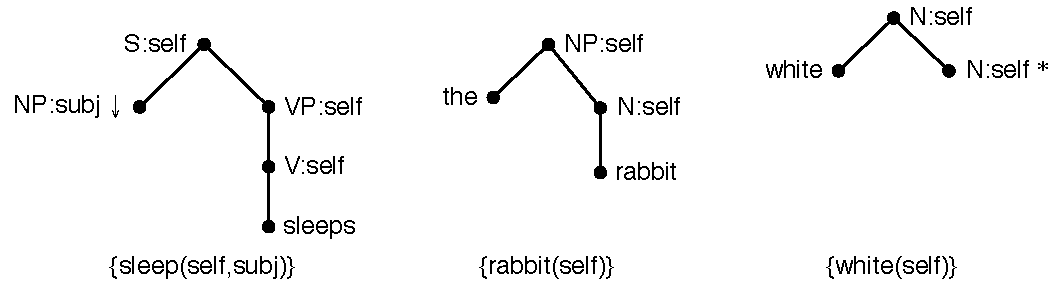
\includegraphics[width=0.75\columnwidth]{pic-grammar}
  \caption{An example grammar in the sentence generation domain.}
  \label{fig:white-rabbit-sleeps-grammar}
\end{figure}

\begin{figure}[t]
  \centering
  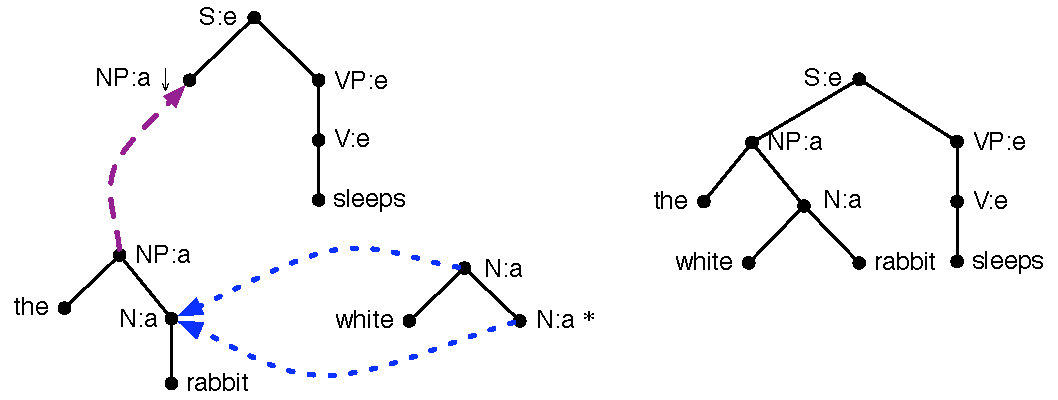
\includegraphics[width=0.75\columnwidth]{pic-derivation}
  \caption{Derivation of ``The white rabbit sleeps.''}
  \label{fig:white-rabbit-sleeps-deriv}
\end{figure}

We can now consider various different algorithms for solving the SPUD
problem. The naive algorithm builds the TAG derivation top-down. In
the example, it starts with the elementary tree for ``sleeps''. This
tree satisfies the need to convey the semantic information, but
introduces a need to generate a noun phrase (NP) for the subject,
which must refer uniquely to the target referent $r_1$. In a second
step, we substitute the tree for ``the rabbit'' into the open NP leaf,
which makes the derivation grammatically complete. Since there are two
different individuals that could be described as ``the
rabbit''---technically, $r_2$ is still a \emph{distractor} (i.e.,
based on the description ``the rabbit'', the hearer might erroneously
think that we're talking about $r_2$ and not $r_1$)---we are still not
finished. To complete the derivation, the tree for ``white'' is added
to the existing structure by an \emph{adjunction} operation, making
the derivation both syntactically and semantically complete. This
search algorithm takes worst-case exponential time because it may have
to consider many combinations of elementary trees; and in fact, the
SPUD problem generalizes the surface realization problem considered by
\citet{KolStr02} and is therefore NP-complete.


\begin{figure}[p]
\centering
\begin{minipage}{0.5\textwidth}
{\small%
\begin{verbatim}
(:action add-sleeps
   :parameters (?u - node
                ?xself - individual
                ?xsubj - individual)
   :precondition
       (and (subst S ?u)
            (referent ?u ?xself)
            (sleep ?xself ?xsubj))
   :effect 
       (and (not (subst S ?u))
            (expressed sleep ?xself ?xsubj)
            (subst NP (subj ?u))
            (referent (subj ?u) ?xsubj)
            (forall (?y - individual)
                (when (not (= ?y ?xself))
                    (distractor (subj ?u) ?y)))))

(:action add-rabbit
   :parameters (?u - node
                ?xself - individual)
   :precondition 
       (and (subst NP ?u)
            (referent ?u ?xself)
            (rabbit ?xself))
   :effect 
       (and (not (subst NP ?u))
            (canadjoin N ?u)
            (forall (?y - individual)
                (when (not (rabbit ?y))
                    (not (distractor ?u ?y))))))

(:action add-white
   :parameters (?u - node
                ?xself - individual)
   :precondition 
       (and (canadjoin N ?u)
            (referent ?u ?xself)
            (rabbit ?xself))
   :effect 
       (forall (?y - individual)
           (when (not (white ?y))
               (not (distractor ?u ?y)))))
\end{verbatim}}%
\end{minipage}
\caption{PDDL actions for generating the sentence ``The white rabbit
sleeps.''}
\label{fig:white-rabbit-as-planning}
\end{figure}

The SPUD system itself worked around this complexity by using a
greedy, incomplete search algorithm. On the other hand,
\citet{KolSto07} present an alternative to controlling the necessary
search, by encoding the generation problem into a planning
problem.\footnote{See \url{http://code.google.com/p/crisp-nlg/} for
  the CRISP system, in which this conversion is implemented.} Each
operator of this planning problem models the addition of some
elementary tree to the TAG derivation. For instance,
Figure~\ref{fig:white-rabbit-as-planning} shows the corresponding PDDL
actions for the above generation task. The \texttt{add-sleeps}
operator represents the addition of the elementary tree for ``sleeps''
to the derivation. $\verb?add-sleep?(\mathsf{root},e,r_1)$ removes the
atom $\mathsf{subst}(S,\mathsf{root})$, which expresses that there is
currently an open substitution node $\mathsf{root}$ with label $S$,
from the planning state and replaces it with an atom
$\mathsf{subst}(NP,\mathsf{subj}(\mathsf{root}))$; here
$\mathsf{subj}(\mathsf{root})$ is meant as shorthand for a fresh
individual name.\footnote{These terms, which are not valid in ordinary
  PDDL, can be eliminated by estimating an upper bound $n$ for the
  plan length, making $n$ copies of each action, ensuring that copy
  $i$ can only be applied in step $i$, and replacing the term
  $\mathsf{subj}(u)$ in an action copy by the constant
  $\mathsf{subj}_i$. Notice that $S$, $NP$, and $N$ are constants.}
At the same time, the operator records that the semantic information
$\mathsf{sleep}(e,r_1)$ has now been expressed, and introduces all
individuals except for $r_1$ as distractors for the new RE at
$\mathsf{subj}(\mathsf{root})$. These distractors can then be removed
by subsequent applications of the other two operators. By assuming an
initial state that encodes the knowledge base and contains an atom
$\mathsf{subst}(S,\emph{root})$, and a goal that contains, among
others, $\forall x \forall y. \neg \mathsf{subst}(x,y)$ and
$\mathsf{expressed}(\emph{sleep},e,r_1)$, a planner will find plans
like the following:
%
\begin{enumerate}
\item $\mathsf{add}\textsf{-}\mathsf{sleeps}(\mathsf{root}, r_1)$,
\item $\mathsf{add}\textsf{-}\mathsf{rabbit}(\mathsf{subj}(\mathsf{root}),r_1)$,
\item $\mathsf{add}\textsf{-}\mathsf{white}(\mathsf{subj}(\mathsf{root}),r_1)$.
\end{enumerate}
%
Using this plan, the grammatical derivation in
Figure~\ref{fig:white-rabbit-sleeps-deriv}, and therefore the
generated sentence ``the white rabbit sleeps'', can be systematically
reconstructed. Thus, we can solve the sentence generation problem via
the detour through planning and bring current search heuristics for
planning to bear on generation.


\subsection{Planning in instruction giving}

Let's now turn to a second recent application of planning in NLG, the
GIVE Challenge (``Generating Instructions in Virtual Environments'';
\citealt{ByrKolStrCasDalMooObe09}). The object of this shared task is
to build an NLG system which produces natural-language instructions
which will guide a human user in performing some task in a virtual
environment.  From an NLG perspective, GIVE makes for an interesting
challenge because it is a theory-neutral task that exercises all
components of an NLG system, and emphasizes the study of communication
in a (simulated) physical environment. Another advantage is that GIVE
makes it possible to connect NLG systems to users over the Internet,
and thus offer cheap access to human experimental subjects. The first
installment of GIVE (GIVE-1) evaluated five NLG systems on the
performance of 1143 users, making it the largest NLG evaluation effort
in terms of human users ever.

\begin{figure}[t]
\centering
%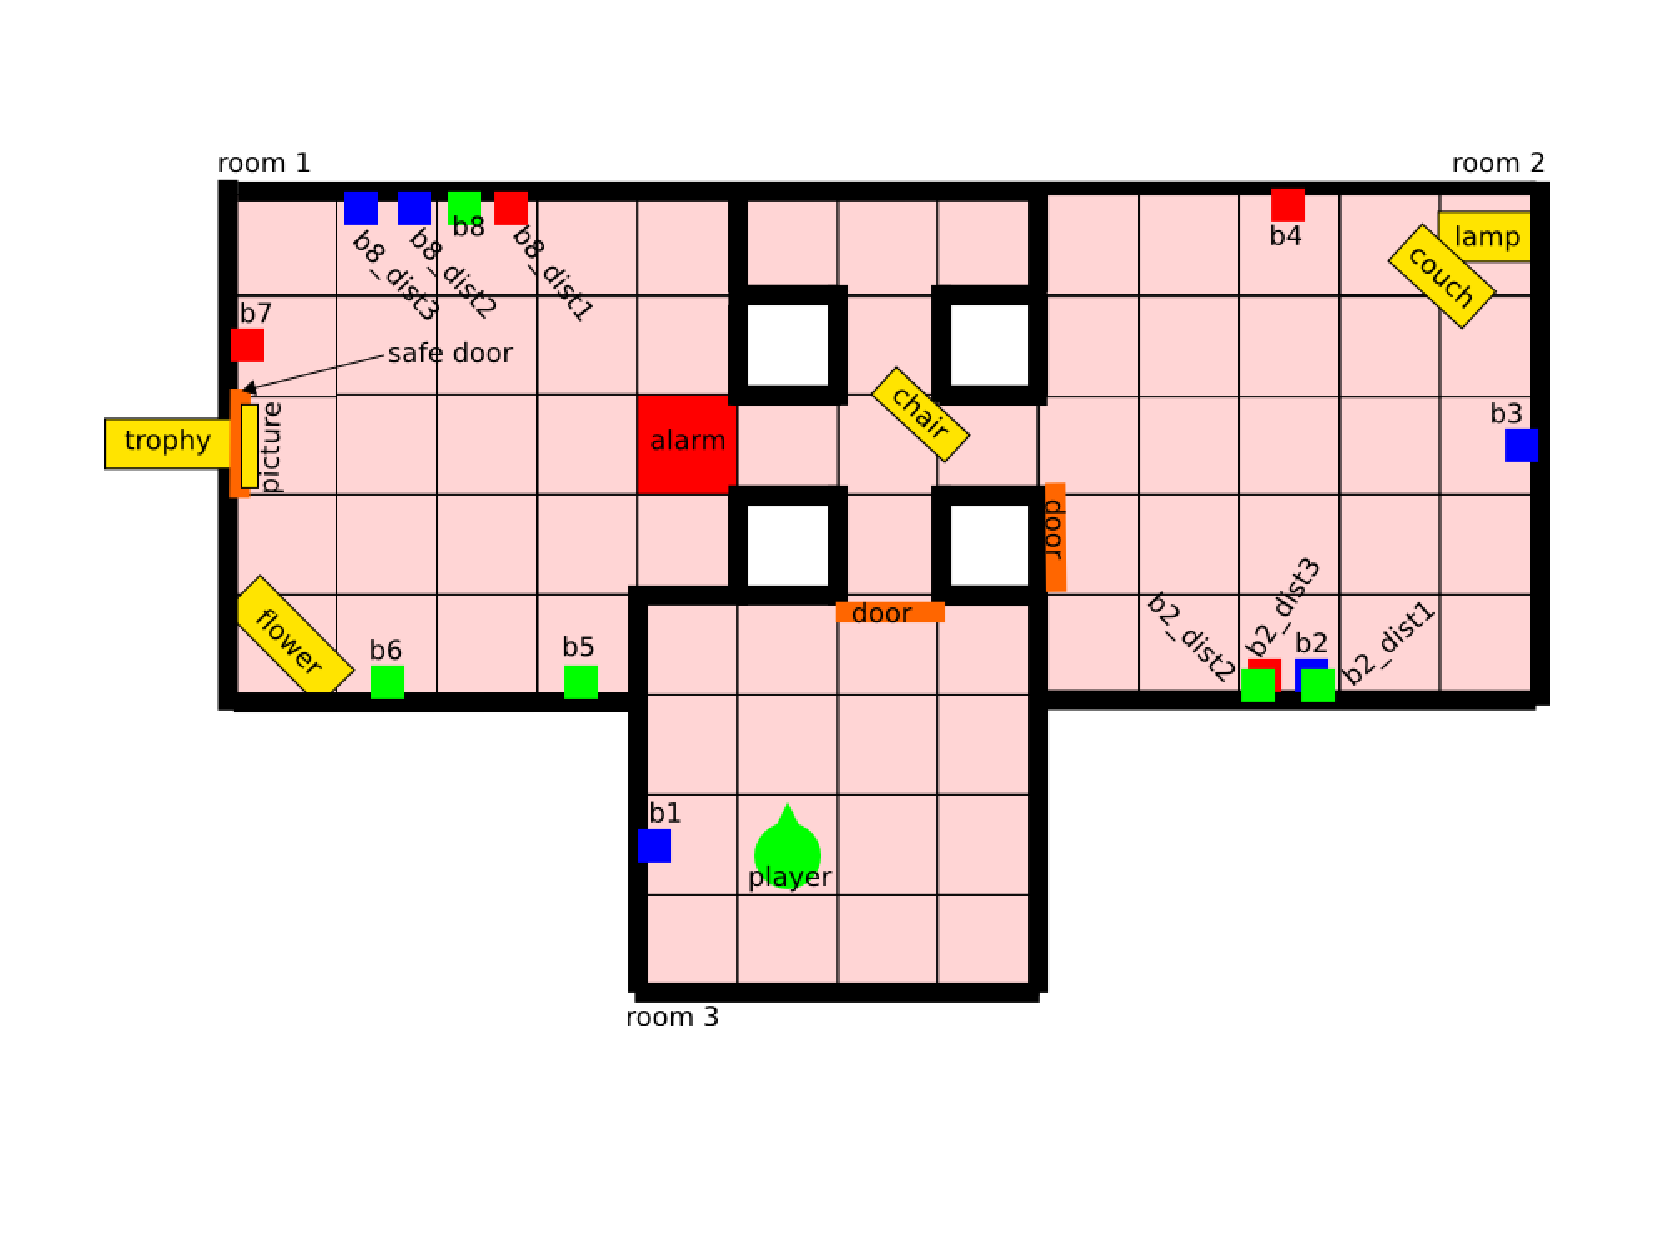
\includegraphics[width=1 \columnwidth]{give_world_no_expl}
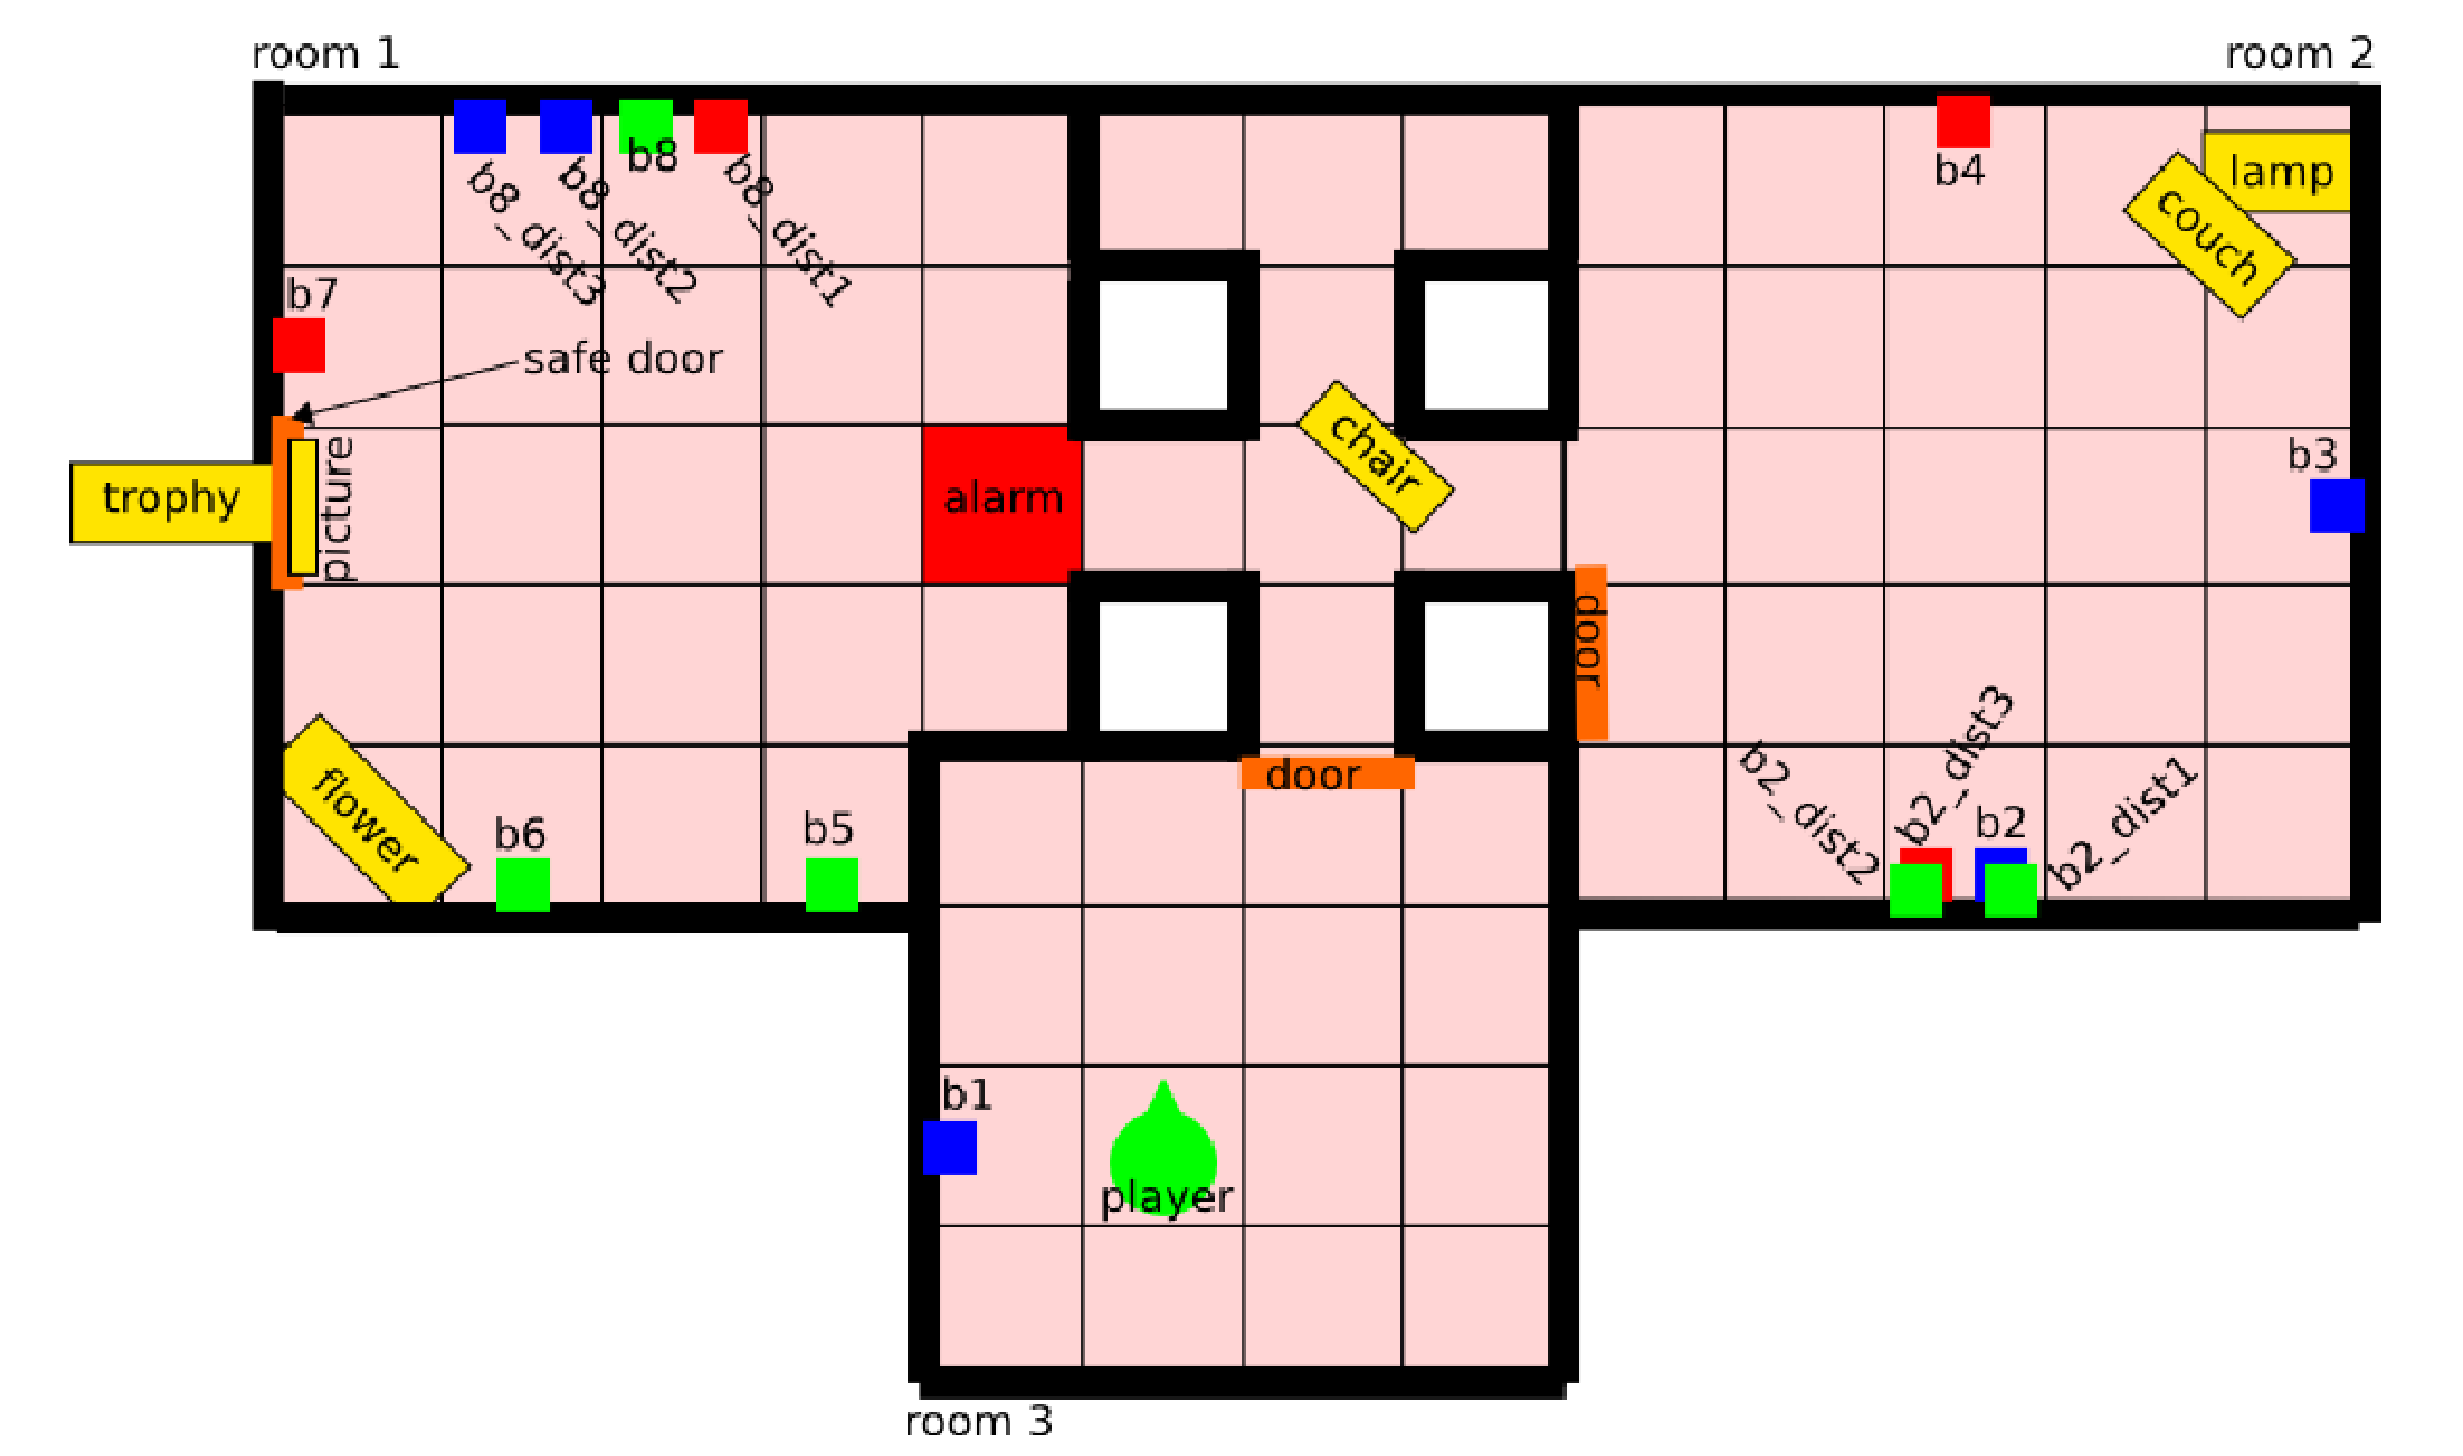
\includegraphics[width=0.75\columnwidth]{give_world_2}
\caption{Map of a GIVE world.}
  \label{fig:give-development-world}
\end{figure}

Planning plays a central role in the GIVE task. To see this, consider
the example GIVE world map in
Figure~\ref{fig:give-development-world}. To simplify both the planning
and the NLG task, this world is discretised into a set of tiles of
equal size.  The user can turn by 90 degree steps in either direction,
and can move from the centre of one tile to the centre of the next
tile, provided the path between two tiles is not blocked. The world
also consists of a set of objects which can be manipulated by the user
in various ways. For instance, in the example world the user's task is
to pick up a trophy in the top left room. The trophy is hidden in a
safe behind a picture; to access it, the user must push certain
buttons in order to move the picture out of the way, open the safe,
and open doors. Figure~\ref{fig:give-planning} shows the encoding of
some of the available GIVE domain actions, in PDDL syntax. In the
example, the shortest plan to solve the task consists of 108 action
steps, with the first few steps as follows:
%
\begin{enumerate}
\item $\mathsf{turn}\textsf{-}\mathsf{left}(\mathsf{north},
\mathsf{west})$,
\item $\mathsf{move}(\mathsf{pos\_5\_2}, \mathsf{pos\_4\_2}, \mathsf{west})$,
\item $\mathsf{manipulate}\textsf{-}\mathsf{b1}\textsf{-}\mathsf{off}\textsf{-}\mathsf{on}(\mathsf{pos\_5\_2})$,
\item $\mathsf{turn}\textsf{-}\mathsf{right}(\mathsf{west}, \mathsf{north})$.
\end{enumerate}

\begin{figure}[p]
\centering
\begin{minipage}{0.5\textwidth}
{\small%
\begin{verbatim}
(:action move
   :parameters (?from - position
                ?to - position
                ?ori - orientation)
   :precondition 
       (and (player-pos ?from) 
            (adjacent ?from ?to ?ori) 
            (player-orient ?ori)
            (not-blocked ?from ?to)
            (not-alarmed ?to))
   :effect 
       (and (not (player-pos ?from))
            (player-pos ?to)))

(:action turn-left
   :parameters (?ori - orientation
                ?newOri - orientation)
   :precondition 
       (and (player-orient ?ori)
            (next-orient-left ?ori ?newOri))
   :effect 
       (and (not (player-orient ?ori))
            (player-orient ?newOri)))

(:action turn-right
   :parameters (?ori - orientation
                ?newOri - orientation)
   :precondition 
       (and (player-orient ?ori)
            (next-orient-right ?ori ?newOri))
   :effect 
       (and (not (player-orient ?ori))
            (player-orient ?newOri)))

(:action manipulate-b1-off-on
   :parameters (?pos - position)
   :precondition 
       (and (state b1 off)
            (player-pos ?pos)
            (position b1 ?pos))
   :effect 
       (and (not (state b1 off))
            (state b1 on)
            (not (state d1 closed))
            (state d1 open) 
            (not (blocked pos_6_5 pos_6_4))
            (not (blocked pos_6_4 pos_6_5))))
\end{verbatim}}%
\end{minipage}
\caption{Some PDDL actions for the GIVE domain.}
\label{fig:give-planning}
\end{figure}

A GIVE NLG system must be able to compute such plans. At a minimum,
the discourse planner will call a planner in order to determine the
content of the instructions that should be presented to the
user. Under this view, the planning problem is very similar to the
Gridworld problem (see, e.g., \citep{Tovey-Koenig:2000}), which also
involves finding a route through a two-dimensional world map with
discrete positions. GIVE tasks are usually much more complex, however,
as illustrated by the above example map: a successful plan must
include steps for pressing buttons in the right order, reasoning about
large numbers of world objects, and navigating through complicated
room shapes. This relatively loose integration of NLG system and
planner is the state of the art of the systems that participated in
GIVE-1.

However, in order to solve the GIVE task in a more satisfying way, we
expect that planning and generation will have to be interleaved more
closely, making the planning a genuine part of the NLG task. For
instance, the NLG system could generate an instruction sequence
starting with ``turn left; walk forward; press the button; turn right;
walk forward; walk forward; turn right; walk forward; walk forward;
turn left; walk forward''. But such instructions are clumsy and
uninteresting; it would be much better to say ``turn around and walk
through the door''. That is, the system should \emph{summarise} plans
by merging multiple action instances into single instructions before
presenting them to the user.\footnote{This task is similar to the
  construction of ``macro'' actions, but is primarily intended for
  plan presentation purposes. See, e.g., \citep{Botea-etal:05} which
  contains a survey of recent approaches for generating macro actions
  in planning.}  Conversely, it may also be necessary to
\emph{elaborate} on a single planning step by expressing it with
several instructions. Having just entered the top left room, it may be
easier for the user to understand the instruction ``walk to the centre
of the room; turn right; now press the green button in front of you'',
rather than the instruction ``press the green button on the wall to
your right''. Furthermore, in order to plan the referring expression
``the green button in front of you'' at a time when the button is not
yet in front of the user, the NLG system must keep track of the
hypothetical changes in what objects are visible to the user. Thus,
the NLG acts of referring and instructing must be tightly integrated
with the modules for plan generation. This makes the GIVE domain
planning problem an integral part of the NLG system, which makes this
a second planning problem of immediate relevance to NLG that is
completely different from the first one.

% It seems to me that this paragraph misses the point. We're not
% trying to sell GIVE as a cool problem here; we take the perspective
% that GIVE exists and has already been shown to be cool, and we only
% talk about solving it here. - AK
%
% From a planning perspective, GIVE imposes very strict runtime
% requirements on the plan generation task: planning must
% happen in real time and the system must respond to a user in a timely
% fashion.  If the system takes too much time deliberating over an
% instruction to give, rather than actually giving this instruction, the
% user may have walked or turned away, thus making the instruction
% invalid.  Furthermore, plan execution monitoring also plays an
% important role in the GIVE problem.  At a high level, the system needs
% to monitor a user's actions and compare them against the generated
% instruction set to determine if the user has correctly followed
% directions or not. In the case of the latter, new instructions may
% have to be generated. In practice, the situation can be quite
% complicated since the mental state of the user is not known and so the
% system must be inferred from observing the user's actions in real
% time. For example, a user directed to ``turn around and walk through
% the door'' may not necessarily perform these actions to the letter,
% i.e., immediately turning 180 degrees and proceeding directly to the
% door. Instead, the user might take a roundabout route through the
% room, eventually exiting out the door.  Although the user's actions do
% not match the generated instructions exactly, they meet the intended
% goal. The system must be able to identify such ``equivalent'' plans
% and not immediately generate new instructions as soon as the user's
% actions have gone off course. Furthermore, a user can communicate
% certain intentions to the system, both through action and
% inaction. For instance, the system should infer that a user has failed
% to follow instructions if the user exits a room when given a directive
% to ``walk to the centre of the room''. The system should also make a
% similar conclusion if a user simply does nothing when given the
% instruction.


%%% Local Variables: 
%%% mode: latex
%%% TeX-master: "manuscript"
%%% End: 
